% Generated by pysimcount.pftchilds -- do not edit; regenerate instead.
% figure: main-t-all-formulas -- Every formula, X-Y-Z grouping, T gates vs n (Clifford+T, every extrapolated step synthesised)
% source: ../np-main/aggregate.json + ../np-main-n9/seed{seed}, ../np-main-n11/seed{seed} (seeds [1, 2, 3, 4, 5, 6, 7, 8, 9, 10]); formulas as in main-cnot-all-formulas.json
% metric=t kind=xyz merged (ct: eps_trotter = 0.0005, eps_synth = 0.0005, simcount template)
% measured n: mean over seeds of the run's T totals; bars min..max over seeds
% extrapolated n: each seed's r = ceil(a_s n^b_s) fitted on n = 5--11; one step built and synthesised per seed at that r; point = mean over seeds, bars min..max
% shown: suzuki4, suzuki6, mo-q6, mo-q14, bm-q10, mo-o8-q21, morales-y8m10, morales-m8
% removed (as in main-cnot-all-formulas.json): lie-trotter, suzuki2, suzuki8
% figure made at git_commit=e5d9ee696f892e28aced765585653760f8a427c4 git_dirty=True
% WARNING: made from uncommitted code; the commit above does not reproduce it.
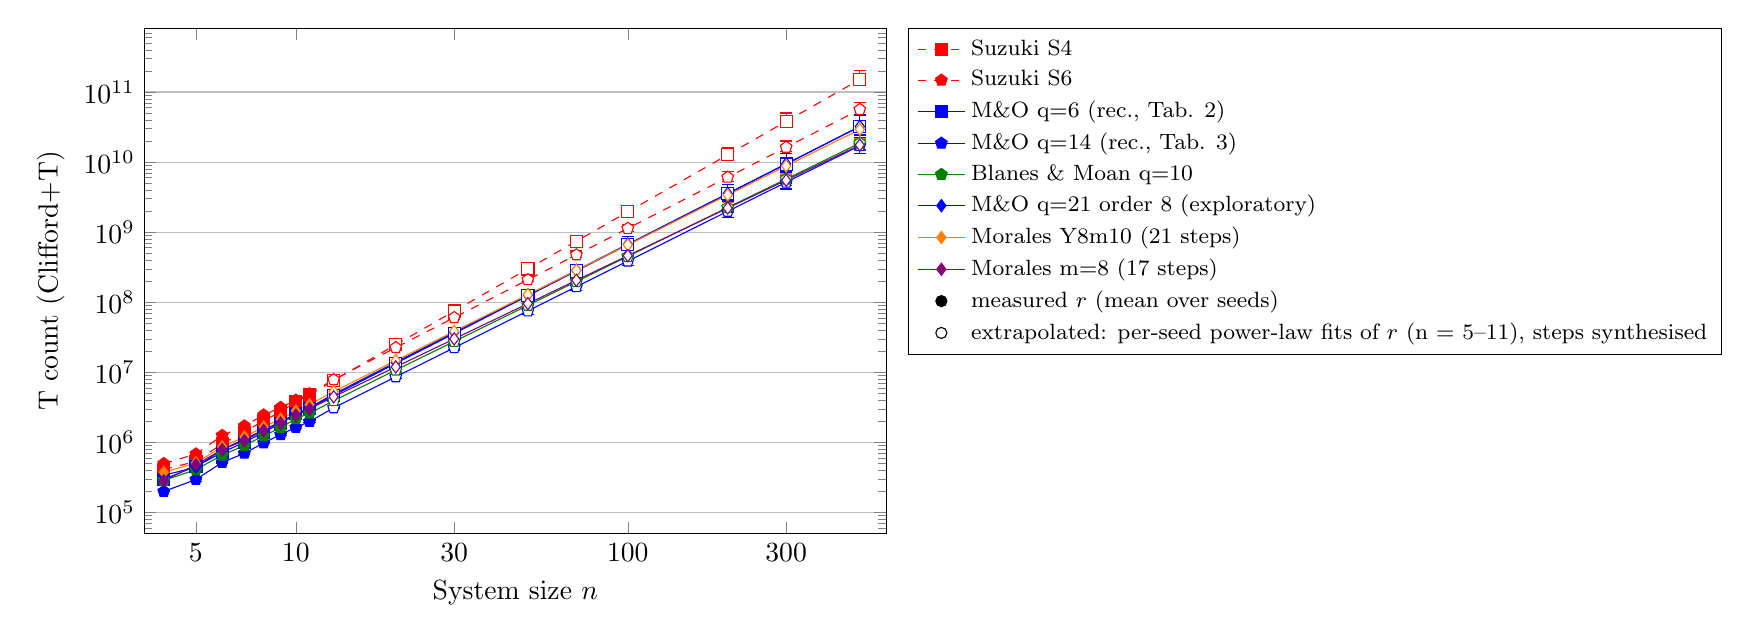
\begin{tikzpicture}
  \begin{loglogaxis}[
    width=11cm, height=8cm,
    xlabel={System size $n$},
    ylabel={T count (Clifford+T)},
    xtick={5,10,30,100,300}, xticklabels={5,10,30,100,300},
    xmin=3.5, xmax=600,
    ymajorgrids=true,
    legend pos=outer north east,
    legend cell align=left,
    legend style={font=\footnotesize},
  ]
    % suzuki4: measured n, mean over seeds, bars min..max over seeds
    \addplot[red, dashed, mark=square*, mark size=2.2pt, mark options={solid, fill=red}, error bars/.cd, y dir=both, y explicit, error bar style={solid}] coordinates {
      (4,410227) += (0,4385) -= (0,12011)
      (5,535141) += (0,32099.4) -= (0,18900.6)
      (6,956087) += (0,61532.8) -= (0,60737.2)
      (7,1.39859e+06) += (0,65506.2) -= (0,81149.8)
      (8,2.05215e+06) += (0,77768.2) -= (0,99723.8)
      (9,2.71254e+06) += (0,149152) -= (0,153838)
      (10,3.81418e+06) += (0,343128) -= (0,119398)
      (11,4.74467e+06) += (0,189676) -= (0,142050)
    };
    \addlegendentry{Suzuki S4}
    % suzuki4: extrapolated, per-seed fitted r, every step synthesised; mean over seeds, bars min..max
    \addplot[red, dashed, mark=square*, mark size=2.2pt, mark options={solid, fill=white}, mark indices={2,...,10}, forget plot, error bars/.cd, y dir=both, y explicit, error bar style={solid}] coordinates {
      (11,4.74467e+06)
      (13,7.66257e+06) += (0,387782) -= (0,206484)
      (20,2.47721e+07) += (0,2.00435e+06) -= (0,1.20859e+06)
      (30,7.47488e+07) += (0,8.81613e+06) -= (0,6.58761e+06)
      (50,2.99557e+08) += (0,4.65816e+07) -= (0,2.86018e+07)
      (70,7.41804e+08) += (0,1.31839e+08) -= (0,7.07925e+07)
      (100,1.95329e+09) += (0,4.06516e+08) -= (0,2.27538e+08)
      (200,1.27159e+10) += (0,3.44947e+09) -= (0,1.88592e+09)
      (300,3.81078e+10) += (0,1.21917e+10) -= (0,6.09671e+09)
      (500,1.5088e+11) += (0,5.3077e+10) -= (0,2.70956e+10)
    };
    % suzuki6: measured n, mean over seeds, bars min..max over seeds
    \addplot[red, dashed, mark=pentagon*, mark size=2.2pt, mark options={solid, fill=red}, error bars/.cd, y dir=both, y explicit, error bar style={solid}] coordinates {
      (4,498655) += (0,32700.8) -= (0,9101.2)
      (5,683636) += (0,27513.8) -= (0,12392.2)
      (6,1.25709e+06) += (0,61765.6) -= (0,83890.4)
      (7,1.71681e+06) += (0,84051) -= (0,117761)
      (8,2.46342e+06) += (0,76166.8) -= (0,20335.2)
      (9,3.14791e+06) += (0,160987) -= (0,93103.2)
      (10,4.01292e+06) += (0,303067) -= (0,211911)
      (11,4.938e+06) += (0,216951) -= (0,170603)
    };
    \addlegendentry{Suzuki S6}
    % suzuki6: extrapolated, per-seed fitted r, every step synthesised; mean over seeds, bars min..max
    \addplot[red, dashed, mark=pentagon*, mark size=2.2pt, mark options={solid, fill=white}, mark indices={2,...,10}, forget plot, error bars/.cd, y dir=both, y explicit, error bar style={solid}] coordinates {
      (11,4.938e+06)
      (13,7.85273e+06) += (0,300450) -= (0,160976)
      (20,2.25571e+07) += (0,1.11956e+06) -= (0,1.00763e+06)
      (30,6.05362e+07) += (0,3.59495e+06) -= (0,2.84472e+06)
      (50,2.09429e+08) += (0,1.94953e+07) -= (0,1.38993e+07)
      (70,4.74592e+08) += (0,6.38993e+07) -= (0,3.83182e+07)
      (100,1.13273e+09) += (0,1.64668e+08) -= (0,1.01944e+08)
      (200,6.08751e+09) += (0,1.27029e+09) -= (0,7.27509e+08)
      (300,1.62764e+10) += (0,3.70913e+09) -= (0,2.14677e+09)
      (500,5.631e+10) += (0,1.54407e+10) -= (0,8.83844e+09)
    };
    % mo-q6: measured n, mean over seeds, bars min..max over seeds
    \addplot[blue, solid, mark=square*, mark size=2.2pt, mark options={solid, fill=blue}, error bars/.cd, y dir=both, y explicit, error bar style={solid}] coordinates {
      (4,298204) += (0,16516.4) -= (0,33723.6)
      (5,454337) += (0,24967.2) -= (0,48760.8)
      (6,719342) += (0,24989.6) -= (0,41182.4)
      (7,1.00507e+06) += (0,53081.4) -= (0,64378.6)
      (8,1.38971e+06) += (0,165321) -= (0,79490.8)
      (9,1.87541e+06) += (0,104483) -= (0,135387)
      (10,2.57989e+06) += (0,145168) -= (0,180656)
      (11,3.07213e+06) += (0,328987) -= (0,277257)
    };
    \addlegendentry{M\&O q=6 (rec., Tab. 2)}
    % mo-q6: extrapolated, per-seed fitted r, every step synthesised; mean over seeds, bars min..max
    \addplot[blue, solid, mark=square*, mark size=2.2pt, mark options={solid, fill=white}, mark indices={2,...,10}, forget plot, error bars/.cd, y dir=both, y explicit, error bar style={solid}] coordinates {
      (11,3.07213e+06)
      (13,4.68293e+06) += (0,356548) -= (0,198754)
      (20,1.33975e+07) += (0,1.57555e+06) -= (0,835830)
      (30,3.58209e+07) += (0,5.86251e+06) -= (0,3.55025e+06)
      (50,1.23593e+08) += (0,2.50475e+07) -= (0,1.49872e+07)
      (70,2.79089e+08) += (0,7.04831e+07) -= (0,4.14157e+07)
      (100,6.61509e+08) += (0,1.94197e+08) -= (0,1.14688e+08)
      (200,3.52821e+09) += (0,1.26118e+09) -= (0,7.4489e+08)
      (300,9.37974e+09) += (0,3.79409e+09) -= (0,2.16652e+09)
      (500,3.21589e+10) += (0,1.48961e+10) -= (0,8.4356e+09)
    };
    % mo-q14: measured n, mean over seeds, bars min..max over seeds
    \addplot[blue, solid, mark=pentagon*, mark size=2.2pt, mark options={solid, fill=blue}, error bars/.cd, y dir=both, y explicit, error bar style={solid}] coordinates {
      (4,199644) += (0,156) -= (0,284)
      (5,295456) += (0,15464) -= (0,15704)
      (6,517803) += (0,21981.2) -= (0,9898.8)
      (7,700110) += (0,16304) -= (0,25074)
      (8,982626) += (0,25418.4) -= (0,17001.6)
      (9,1.29212e+06) += (0,59288.2) -= (0,40565.8)
      (10,1.63772e+06) += (0,50796.4) -= (0,66587.6)
      (11,1.98699e+06) += (0,75316.4) -= (0,57607.6)
    };
    \addlegendentry{M\&O q=14 (rec., Tab. 3)}
    % mo-q14: extrapolated, per-seed fitted r, every step synthesised; mean over seeds, bars min..max
    \addplot[blue, solid, mark=pentagon*, mark size=2.2pt, mark options={solid, fill=white}, mark indices={2,...,10}, forget plot, error bars/.cd, y dir=both, y explicit, error bar style={solid}] coordinates {
      (11,1.98699e+06)
      (13,3.11874e+06) += (0,57718.4) -= (0,105462)
      (20,8.61978e+06) += (0,566221) -= (0,428091)
      (30,2.2459e+07) += (0,2.19943e+06) -= (0,1.58811e+06)
      (50,7.52655e+07) += (0,9.82788e+06) -= (0,7.79298e+06)
      (70,1.66795e+08) += (0,2.71474e+07) -= (0,2.02453e+07)
      (100,3.86553e+08) += (0,7.14752e+07) -= (0,5.46946e+07)
      (200,1.98691e+09) += (0,4.88484e+08) -= (0,3.55086e+08)
      (300,5.16555e+09) += (0,1.40651e+09) -= (0,1.03303e+09)
      (500,1.71426e+10) += (0,5.38038e+09) -= (0,3.83706e+09)
    };
    % bm-q10: measured n, mean over seeds, bars min..max over seeds
    \addplot[green!50!black, solid, mark=pentagon*, mark size=2.2pt, mark options={solid, fill=green!50!black}, error bars/.cd, y dir=both, y explicit, error bar style={solid}] coordinates {
      (4,287233) += (0,5966.8) -= (0,8617.2)
      (5,408923) += (0,4588.8) -= (0,16769.2)
      (6,658784) += (0,7867.6) -= (0,17360.4)
      (7,901238) += (0,22542) -= (0,24694)
      (8,1.23945e+06) += (0,56480.4) -= (0,33631.6)
      (9,1.62436e+06) += (0,90390.6) -= (0,104629)
      (10,2.1788e+06) += (0,37144.4) -= (0,61775.6)
      (11,2.60871e+06) += (0,138211) -= (0,70676.8)
    };
    \addlegendentry{Blanes \& Moan q=10}
    % bm-q10: extrapolated, per-seed fitted r, every step synthesised; mean over seeds, bars min..max
    \addplot[green!50!black, solid, mark=pentagon*, mark size=2.2pt, mark options={solid, fill=white}, mark indices={2,...,10}, forget plot, error bars/.cd, y dir=both, y explicit, error bar style={solid}] coordinates {
      (11,2.60871e+06)
      (13,3.9301e+06) += (0,68836) -= (0,87804)
      (20,1.0774e+07) += (0,460669) -= (0,649855)
      (30,2.7548e+07) += (0,1.70443e+06) -= (0,1.9026e+06)
      (50,9.03062e+07) += (0,6.58258e+06) -= (0,8.73882e+06)
      (70,1.9751e+08) += (0,1.7158e+07) -= (0,2.14673e+07)
      (100,4.51462e+08) += (0,4.29653e+07) -= (0,5.62649e+07)
      (200,2.24975e+09) += (0,2.68432e+08) -= (0,3.56254e+08)
      (300,5.73099e+09) += (0,7.68518e+08) -= (0,1.04131e+09)
      (500,1.86331e+10) += (0,2.68049e+09) -= (0,3.81581e+09)
    };
    % mo-o8-q21: measured n, mean over seeds, bars min..max over seeds
    \addplot[blue, solid, mark=diamond*, mark size=2.2pt, mark options={solid, fill=blue}, error bars/.cd, y dir=both, y explicit, error bar style={solid}] coordinates {
      (4,338991) += (0,798.6) -= (0,543.4)
      (5,443831) += (0,29857.2) -= (0,13070.8)
      (6,791120) += (0,35284.4) -= (0,16111.6)
      (7,1.1119e+06) += (0,48135) -= (0,83745)
      (8,1.50621e+06) += (0,35620.2) -= (0,35067.8)
      (9,1.97285e+06) += (0,86982) -= (0,71248)
      (10,2.54893e+06) += (0,177979) -= (0,71636.6)
      (11,3.13956e+06) += (0,105399) -= (0,122217)
    };
    \addlegendentry{M\&O q=21 order 8 (exploratory)}
    % mo-o8-q21: extrapolated, per-seed fitted r, every step synthesised; mean over seeds, bars min..max
    \addplot[blue, solid, mark=diamond*, mark size=2.2pt, mark options={solid, fill=white}, mark indices={2,...,10}, forget plot, error bars/.cd, y dir=both, y explicit, error bar style={solid}] coordinates {
      (11,3.13956e+06)
      (13,4.88976e+06) += (0,56791) -= (0,186319)
      (20,1.39079e+07) += (0,486906) -= (0,907256)
      (30,3.70353e+07) += (0,1.60026e+06) -= (0,3.14339e+06)
      (50,1.2702e+08) += (0,8.2286e+06) -= (0,1.46677e+07)
      (70,2.85327e+08) += (0,2.31775e+07) -= (0,3.56762e+07)
      (100,6.73578e+08) += (0,6.27389e+07) -= (0,1.02361e+08)
      (200,3.56917e+09) += (0,4.59913e+08) -= (0,6.71365e+08)
      (300,9.45042e+09) += (0,1.40818e+09) -= (0,1.97079e+09)
      (500,3.22461e+10) += (0,5.17455e+09) -= (0,7.59363e+09)
    };
    % morales-y8m10: measured n, mean over seeds, bars min..max over seeds
    \addplot[orange, solid, mark=diamond*, mark size=2.2pt, mark options={solid, fill=orange}, error bars/.cd, y dir=both, y explicit, error bar style={solid}] coordinates {
      (4,373838) += (0,393.6) -= (0,350.4)
      (5,509327) += (0,585) -= (0,507)
      (6,864458) += (0,62172.2) -= (0,39345.8)
      (7,1.19952e+06) += (0,67633.6) -= (0,46602.4)
      (8,1.66587e+06) += (0,68593.4) -= (0,61034.6)
      (9,2.15577e+06) += (0,61279.2) -= (0,87138.8)
      (10,2.81799e+06) += (0,237300) -= (0,154036)
      (11,3.46189e+06) += (0,101580) -= (0,101050)
    };
    \addlegendentry{Morales Y8m10 (21 steps)}
    % morales-y8m10: extrapolated, per-seed fitted r, every step synthesised; mean over seeds, bars min..max
    \addplot[orange, solid, mark=diamond*, mark size=2.2pt, mark options={solid, fill=white}, mark indices={2,...,10}, forget plot, error bars/.cd, y dir=both, y explicit, error bar style={solid}] coordinates {
      (11,3.46189e+06)
      (13,5.32463e+06) += (0,272075) -= (0,227581)
      (20,1.47085e+07) += (0,1.14689e+06) -= (0,1.13279e+06)
      (30,3.84186e+07) += (0,3.78324e+06) -= (0,3.5671e+06)
      (50,1.28596e+08) += (0,1.83792e+07) -= (0,1.61923e+07)
      (70,2.84865e+08) += (0,4.67169e+07) -= (0,4.26348e+07)
      (100,6.59306e+08) += (0,1.2942e+08) -= (0,1.13282e+08)
      (200,3.39046e+09) += (0,8.63829e+08) -= (0,7.1373e+08)
      (300,8.80299e+09) += (0,2.42332e+09) -= (0,2.02459e+09)
      (500,2.92891e+10) += (0,9.53382e+09) -= (0,7.5792e+09)
    };
    % morales-m8: measured n, mean over seeds, bars min..max over seeds
    \addplot[violet, solid, mark=diamond*, mark size=2.2pt, mark options={solid, fill=violet}, error bars/.cd, y dir=both, y explicit, error bar style={solid}] coordinates {
      (4,283483) += (0,15076.8) -= (0,14775.2)
      (5,480273) += (0,27567) -= (0,4293)
      (6,790926) += (0,38574) -= (0,5206)
      (7,1.06227e+06) += (0,12522.6) -= (0,45515.4)
      (8,1.48074e+06) += (0,49073) -= (0,12907)
      (9,1.89288e+06) += (0,79598.4) -= (0,47401.6)
      (10,2.4461e+06) += (0,66195.6) -= (0,18780.4)
      (11,3.00394e+06) += (0,9119.6) -= (0,60158.4)
    };
    \addlegendentry{Morales m=8 (17 steps)}
    % morales-m8: extrapolated, per-seed fitted r, every step synthesised; mean over seeds, bars min..max
    \addplot[violet, solid, mark=diamond*, mark size=2.2pt, mark options={solid, fill=white}, mark indices={2,...,10}, forget plot, error bars/.cd, y dir=both, y explicit, error bar style={solid}] coordinates {
      (11,3.00394e+06)
      (13,4.48114e+06) += (0,71643.2) -= (0,105161)
      (20,1.19454e+07) += (0,365553) -= (0,348003)
      (30,3.00095e+07) += (0,1.1417e+06) -= (0,1.11385e+06)
      (50,9.5688e+07) += (0,5.37813e+06) -= (0,4.85e+06)
      (70,2.05711e+08) += (0,1.29501e+07) -= (0,1.22873e+07)
      (100,4.61972e+08) += (0,3.26388e+07) -= (0,3.73721e+07)
      (200,2.2065e+09) += (0,1.93245e+08) -= (0,2.24446e+08)
      (300,5.51227e+09) += (0,5.39536e+08) -= (0,6.30311e+08)
      (500,1.75035e+10) += (0,1.90596e+09) -= (0,2.33772e+09)
    };
    \addlegendimage{only marks, black, mark=*, mark options={solid, fill=black}}
    \addlegendentry{measured $r$ (mean over seeds)}
    \addlegendimage{only marks, black, mark=*, mark options={solid, fill=white}}
    \addlegendentry{extrapolated: per-seed power-law fits of $r$ (n = 5--11), steps synthesised}
  \end{loglogaxis}
\end{tikzpicture}
